For understanding when a new state has occurred a method for detecting this has to be developed. The method will consist of three steps:

\begin{enumerate}
\setlength{\itemsep}{0mm}
	\item Detect if human interaction has occurred.
	\item Wait until balls are laying still.
	\item If human interaction occured, then detect if ball position or number of ball changed.
\end{enumerate}


\subsection{Human interaction detection}
The first step is to detect weather or not the cloth is occluded. This occlusion could be caused by human interaction or foreign object placed within the cloth of the table. Detection will be used before finding position of balls. If the cloth is detected to be occluded then there will be no detection of balls before the table is no longer interacted with. This will bring down faulty detections caused by cue or foreign objects.\\

When the table is detected in calibration, as described in section \ref{sec:table-locate}, a mask for the cloth is made. This mask is made from a contour which has many different properties such as area and perimeter. These properties can be used when identifying if occlusions are present. By comparing the current image mask together with the mask made in the calibration and finding the difference in area or perimeter, detection should be possible.\\

For this purpose of this method only foreign object introduced from the edge and in will be considered as a foreign object. Therefore a que from the edge of the table would be detected, but a ball or foreign object laying on the table will not.

Occlusion area factor:
\begin{equation}
\lambda = \frac{A_{current}}{A_{calibrated}}
\label{eq:area}
\end{equation}

Occlusion perimeter factor:
\begin{equation}
\kappa = \frac{P_{current}}{P_{calibrated}}
\label{eq:perimeter}
\end{equation}

\textbf{Test Image With Values and Factors:}\\
\begin{tabular}{|l|c|c|l|l|c|}
\hline - & Image & Mask & A \& $\lambda$ & P \& $\kappa$ & Occlusion \\ 
\hline

\multirow{4}{*}{Calibrated.} & \multirow{4}{*}{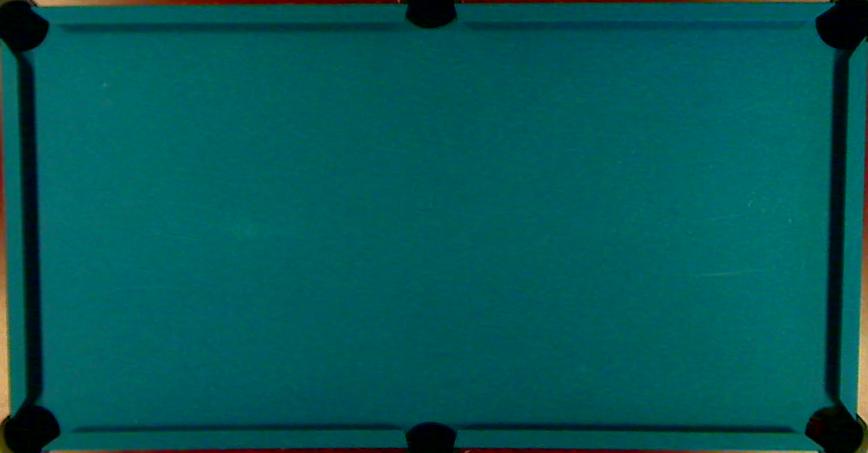
\includegraphics[scale=0.1]{../images/1/calibimg.png}} & \multirow{4}{*}{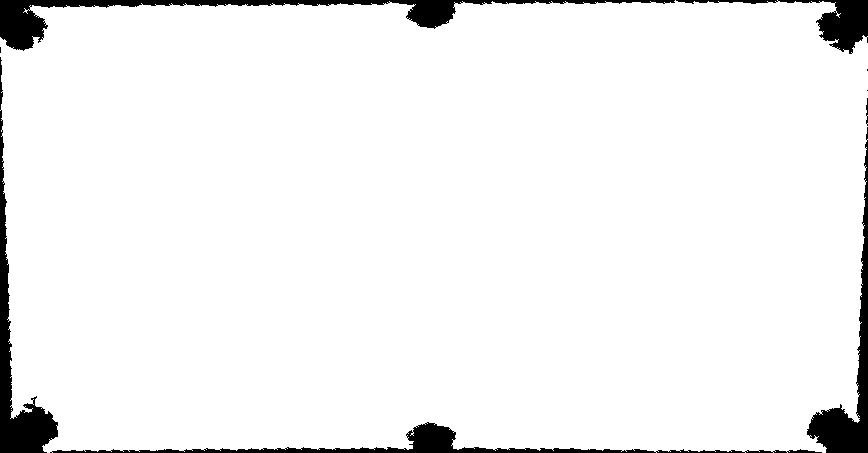
\includegraphics[scale=0.1]{../images/1/calibmask.png}} & A = 369861 & P = 3153  & \multirow{4}{*}{}\\  
& & & & & \\
&&&&&\\
&&&&&\\
\hline

\multirow{4}{*}{Empty table.} & \multirow{4}{*}{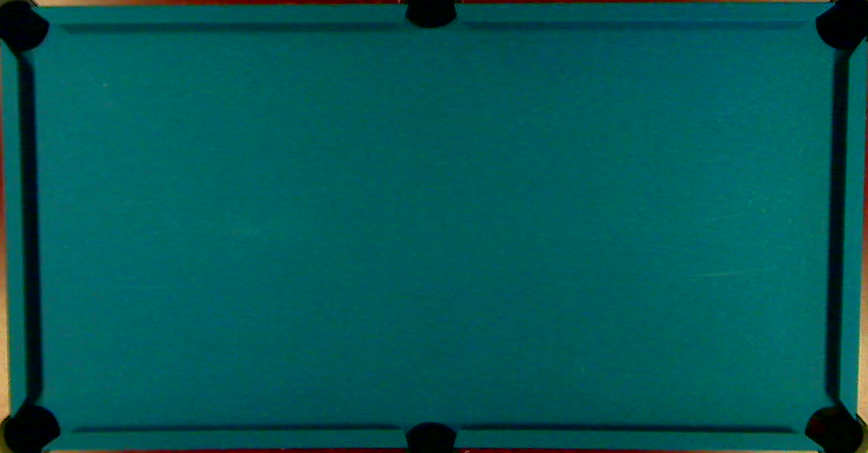
\includegraphics[scale=0.1]{../images/1/0_img.png}} & \multirow{4}{*}{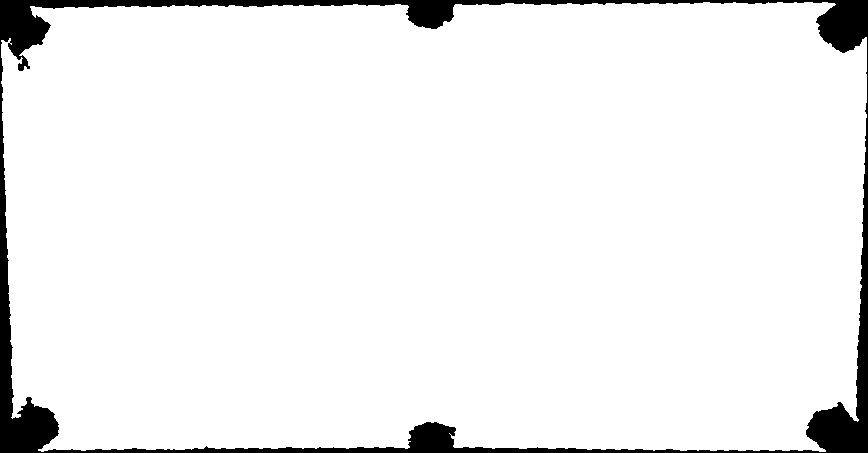
\includegraphics[scale=0.1]{../images/1/0_mask.png}} & A = 369518 & P = 3185 & \multirow{4}{*}{}\\  
& & & $\lambda$ = 0.9991 & $\kappa$ = 1.0099 & \\
&&&&&\\
&&&&&\\
\hline

\multirow{4}{*}{With balls.} & \multirow{4}{*}{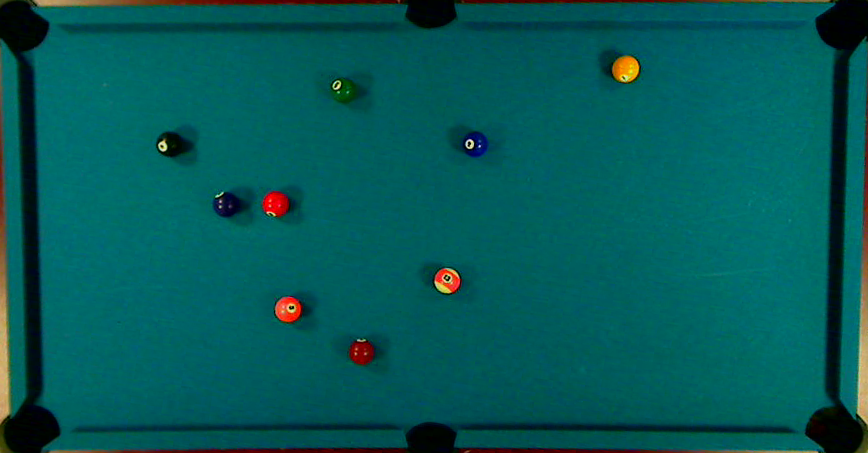
\includegraphics[scale=0.1]{../images/1/1_img.png}} & \multirow{4}{*}{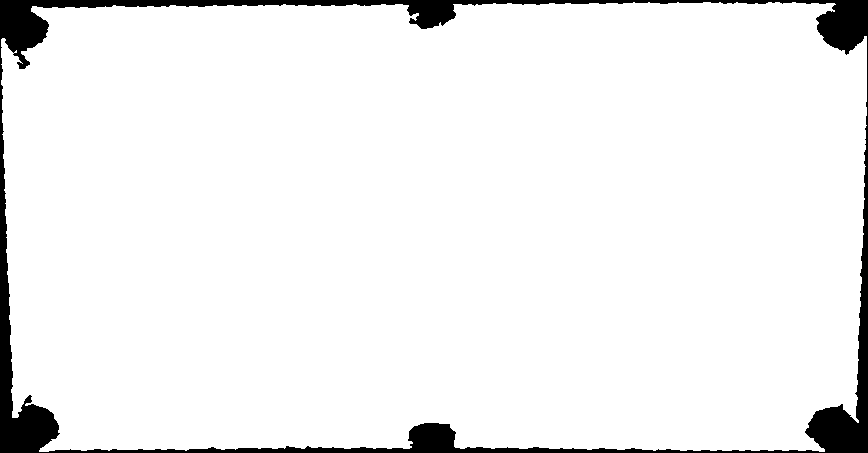
\includegraphics[scale=0.1]{../images/1/1_mask.png}} & A = 369852 & P = 3193 & \multirow{4}{*}{}\\ 
& & & $\lambda$ = 1 & $\kappa$ = 1.0127 & \\
&&&&&\\
&&&&&\\
\hline

\multirow{4}{*}{With person.} & \multirow{4}{*}{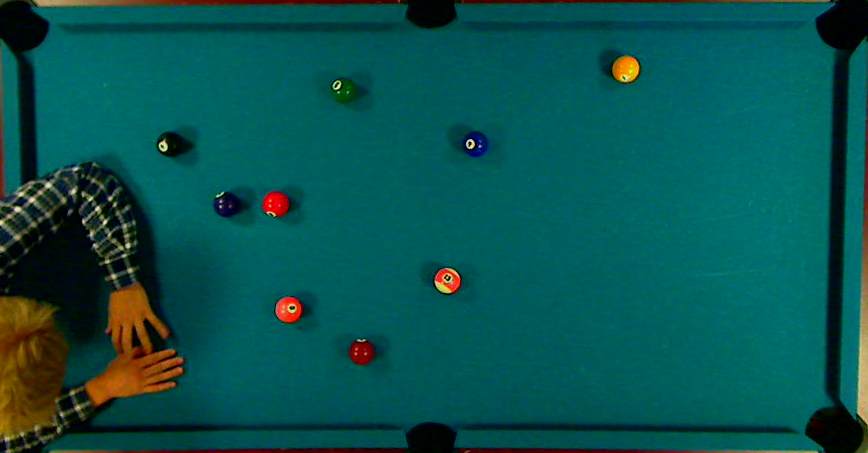
\includegraphics[scale=0.1]{../images/1/2_img.png}} & \multirow{4}{*}{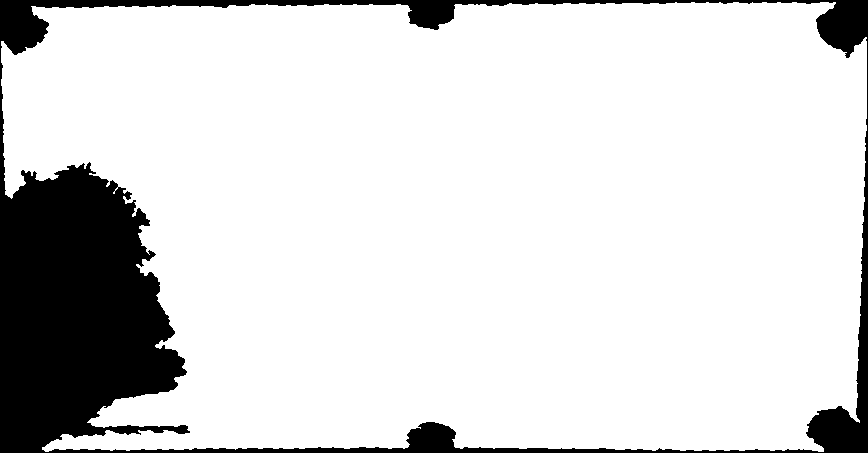
\includegraphics[scale=0.1]{../images/1/2_mask.png}} & A = 334652 & P = 3866 & \multirow{4}{*}{\checkmark}\\  
& & & $\lambda$ = 0.9048 & $\kappa$ = 1.2258 & \\
&&&&&\\
&&&&&\\
\hline

\multirow{4}{*}{Que on table I.} & \multirow{4}{*}{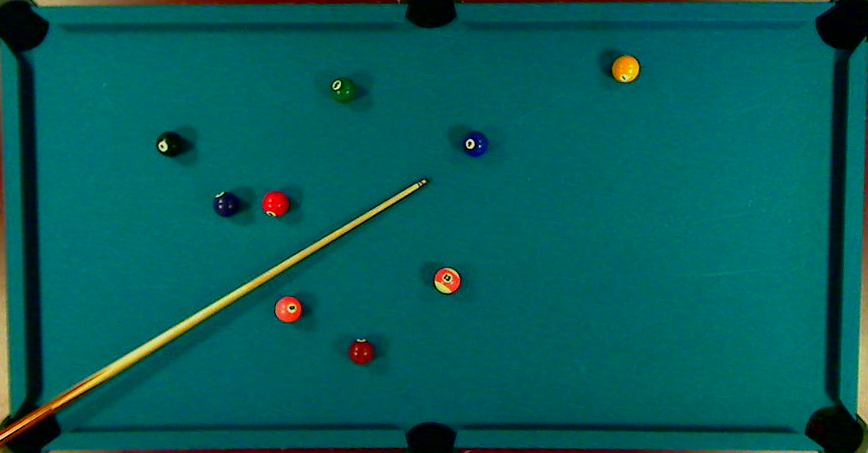
\includegraphics[scale=0.1]{../images/1/3_img.png}} & \multirow{4}{*}{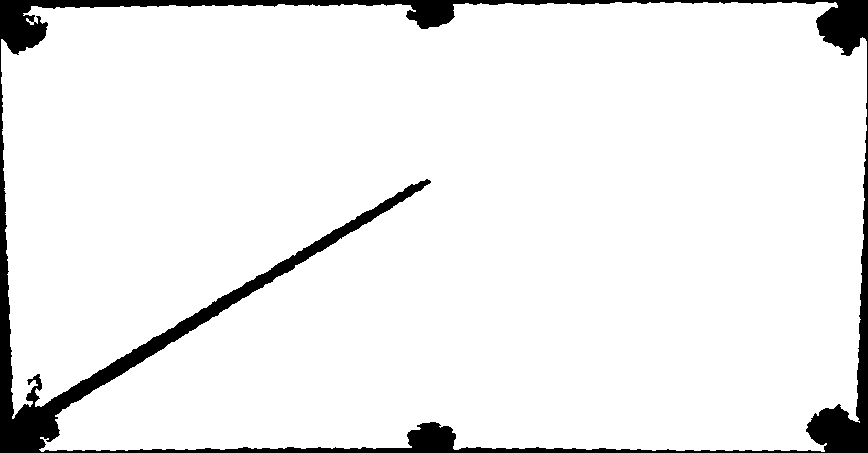
\includegraphics[scale=0.1]{../images/1/3_mask.png}} & A = 364515 & P = 4287 & \multirow{4}{*}{\checkmark}\\  
& & & $\lambda$ = 0.9855 & $\kappa$ = 1.3594 & \\
&&&&&\\
&&&&&\\
\hline

\multirow{4}{*}{Que on table II.} & \multirow{4}{*}{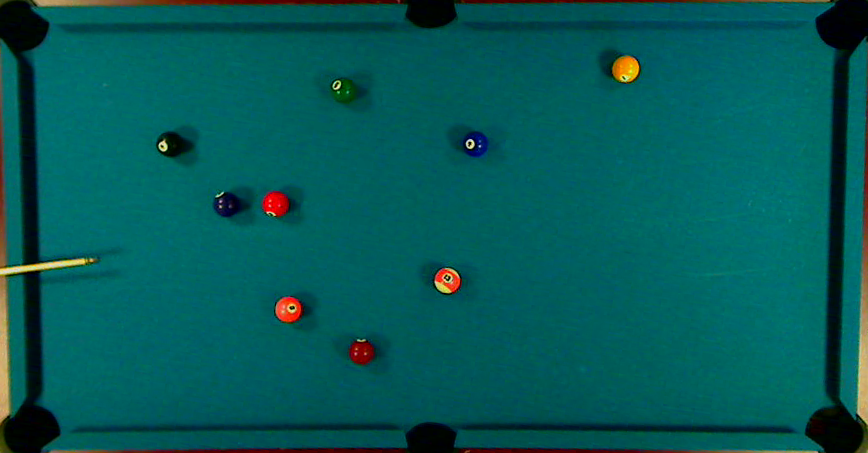
\includegraphics[scale=0.1]{../images/1/4_img.png}} & \multirow{4}{*}{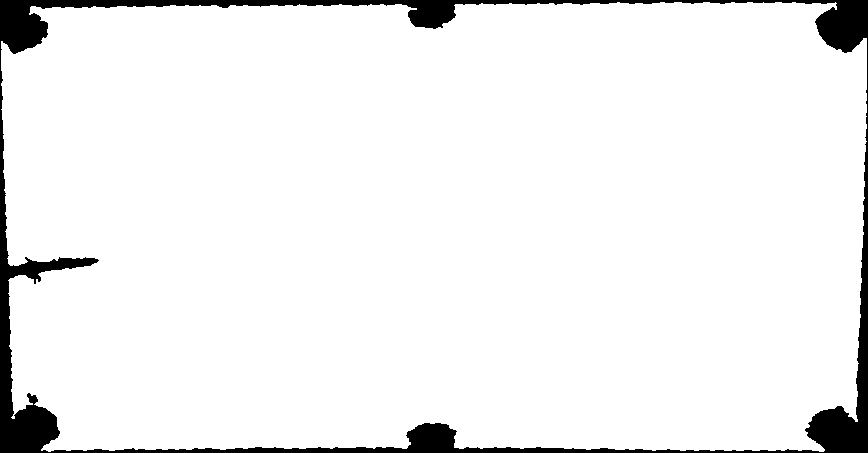
\includegraphics[scale=0.1]{../images/1/4_mask.png}} & A = 368846 & P = 3324 & \multirow{4}{*}{\checkmark}\\  
& & & $\lambda$ = 0.9973 & $\kappa$ = 1.0541 & \\
&&&&&\\
&&&&&\\
\hline

\multirow{4}{*}{Que on table III.} & \multirow{4}{*}{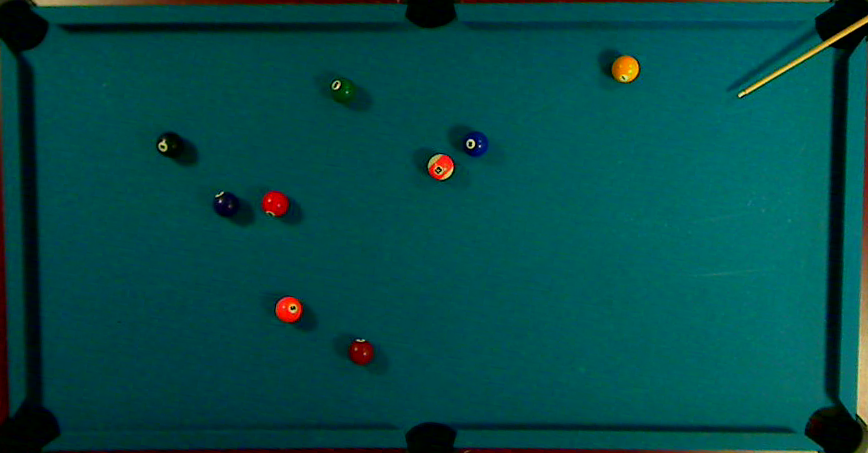
\includegraphics[scale=0.1]{../images/1/11_img.png}} & \multirow{4}{*}{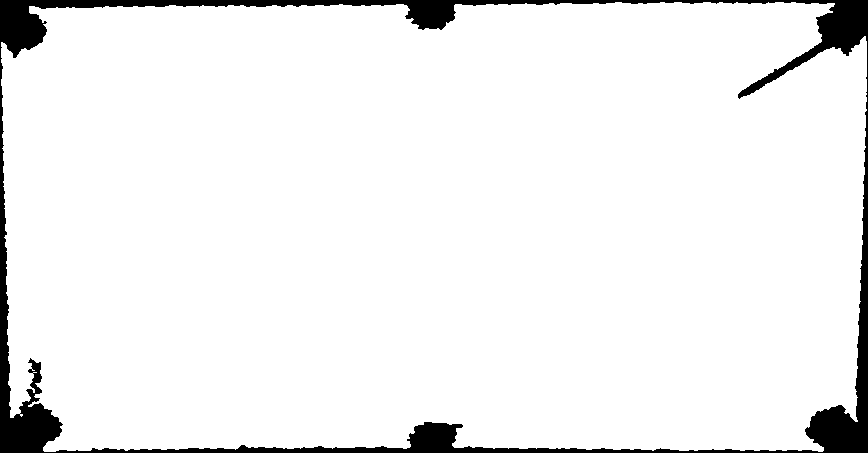
\includegraphics[scale=0.1]{../images/1/11_mask.png}} & A = 368555 & P = 3566 & \multirow{4}{*}{\checkmark}\\ 
& & & $\lambda$ = 0.9965 & $\kappa$ = 1.1307 & \\
&&&&&\\
&&&&&\\
\hline
\end{tabular} 

\begin{tabular}{|l|c|c|l|l|c|}
\hline - & Image & Mask & A \& $\lambda$ & P \& $\kappa$ & Occlusion \\ 
\hline


\multirow{4}{*}{Que on table IV.} & \multirow{4}{*}{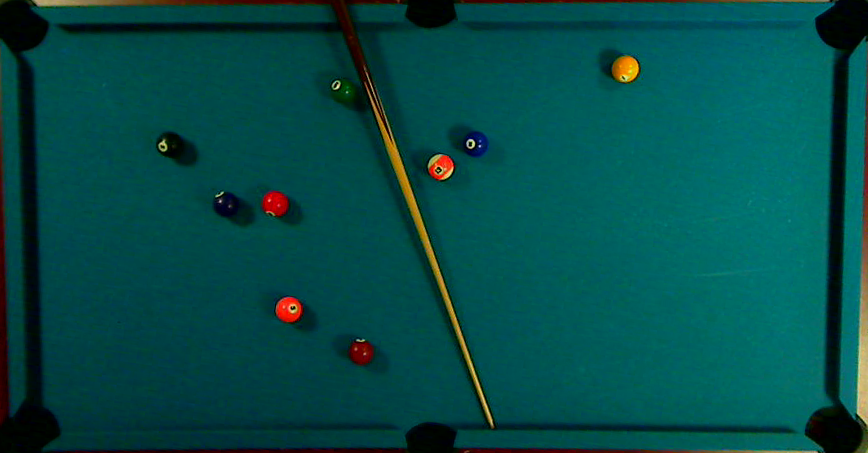
\includegraphics[scale=0.1]{../images/1/12_img.png}} & \multirow{4}{*}{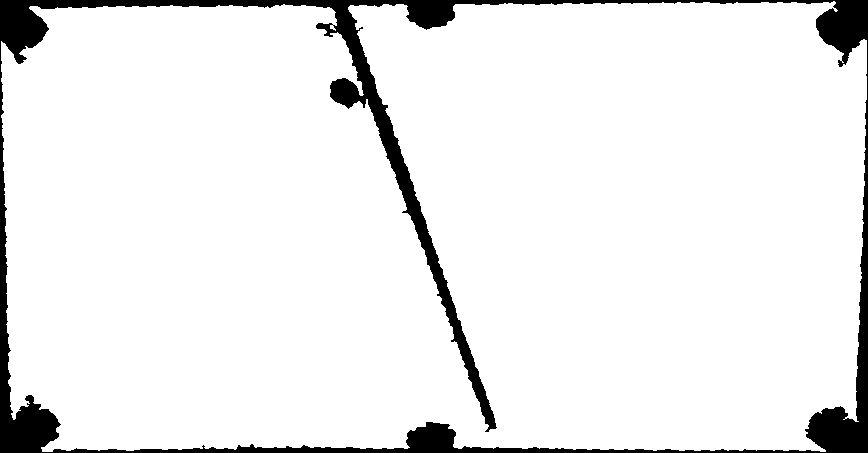
\includegraphics[scale=0.1]{../images/1/12_mask.png}} & A = 362749 & P = 4458 & \multirow{4}{*}{\checkmark}\\ 
& & & $\lambda$ = 0.9808 & $\kappa$ = 1.4138 & \\
&&&&&\\
&&&&&\\
\hline

\multirow{4}{*}{Chair on table.} & \multirow{4}{*}{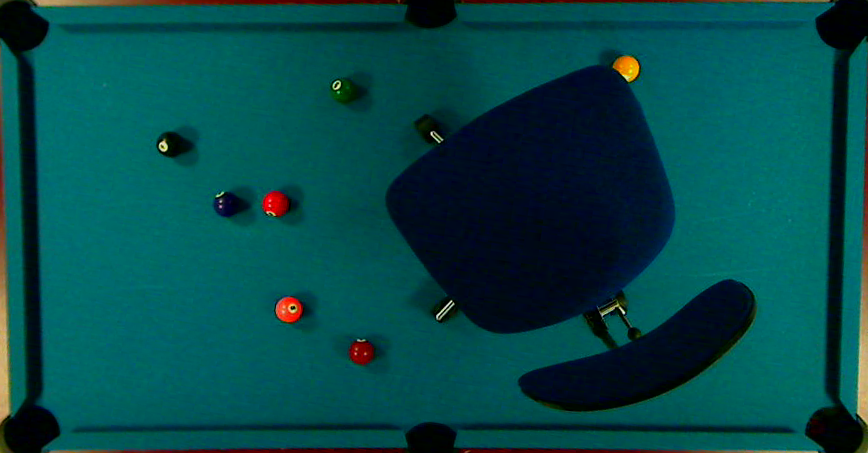
\includegraphics[scale=0.1]{../images/1/5_img.png}} & \multirow{4}{*}{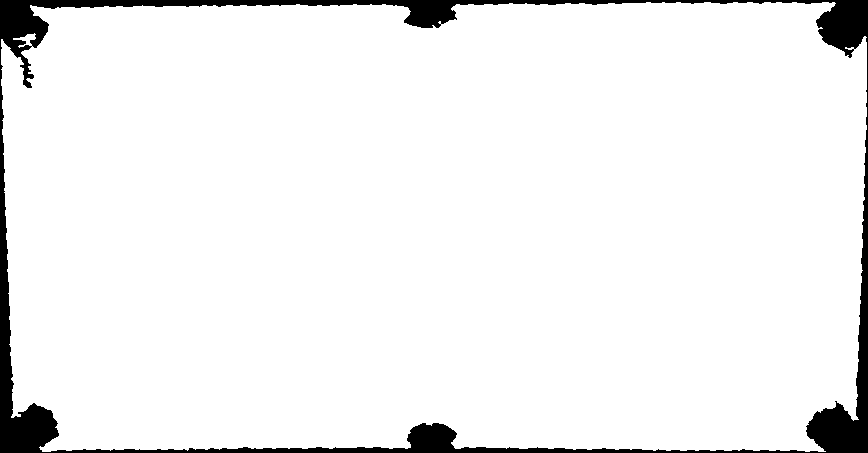
\includegraphics[scale=0.1]{../images/1/5_mask.png}} & A = 369881 & P = 3336 & \multirow{4}{*}{}\\  
& & & $\lambda$ = 1 & $\kappa$ = 1.0578 & \\
&&&&&\\
&&&&&\\
\hline

\multirow{4}{*}{Shadow.} & \multirow{4}{*}{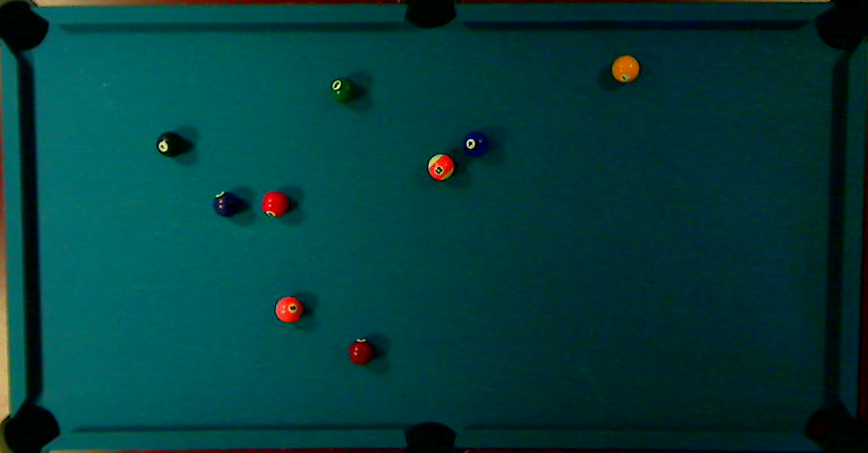
\includegraphics[scale=0.1]{../images/1/6_img.png}} & \multirow{4}{*}{
\includegraphics[scale=0.1]{../images/1/6_mask.png}} & A = 366844 & P = 3780 & \multirow{4}{*}{}\\ 
& & & $\lambda$ = 0.9918 & $\kappa$ = 1.1986 & \\
&&&&&\\
&&&&&\\
\hline

\multirow{4}{*}{Lighting I.} & \multirow{4}{*}{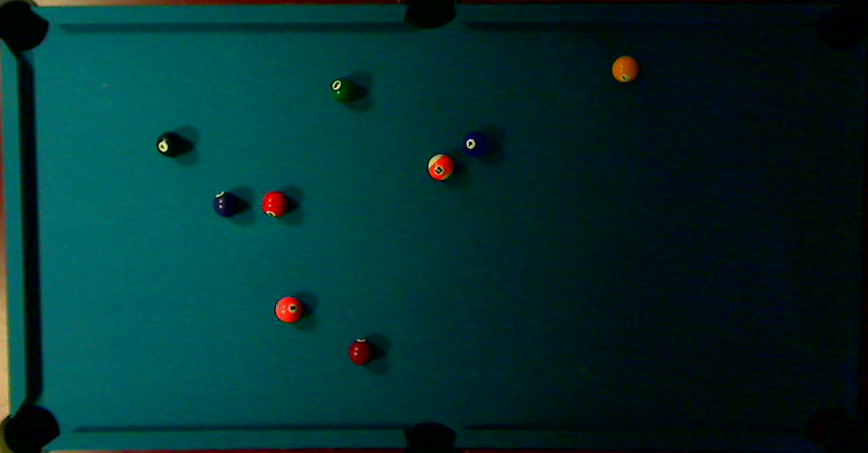
\includegraphics[scale=0.1]{../images/1/7_img.png}} & \multirow{4}{*}{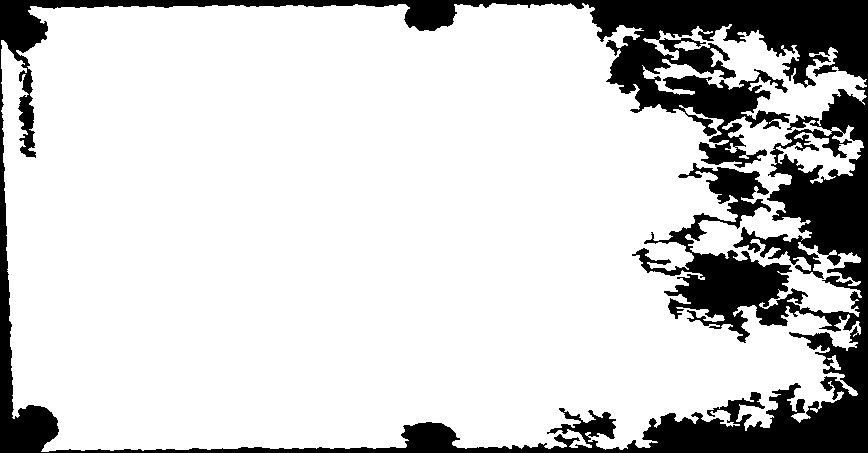
\includegraphics[scale=0.1]{../images/1/7_mask.png}} & A = 314105 & P = 12473 & \multirow{4}{*}{}\\ 
& & & $\lambda$ = 0.8493 & $\kappa$ = 3.9550 & \\
&&&&&\\
&&&&&\\
\hline

\multirow{4}{*}{Lighting II.} & \multirow{4}{*}{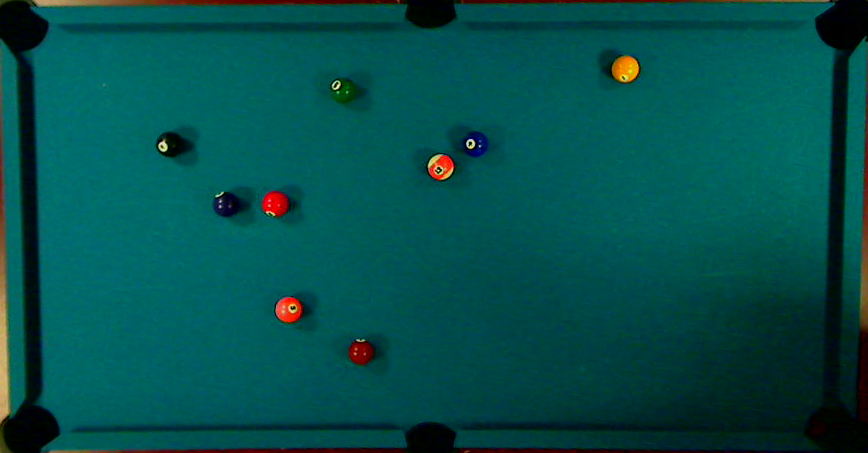
\includegraphics[scale=0.1]{../images/1/8_img.png}} & \multirow{4}{*}{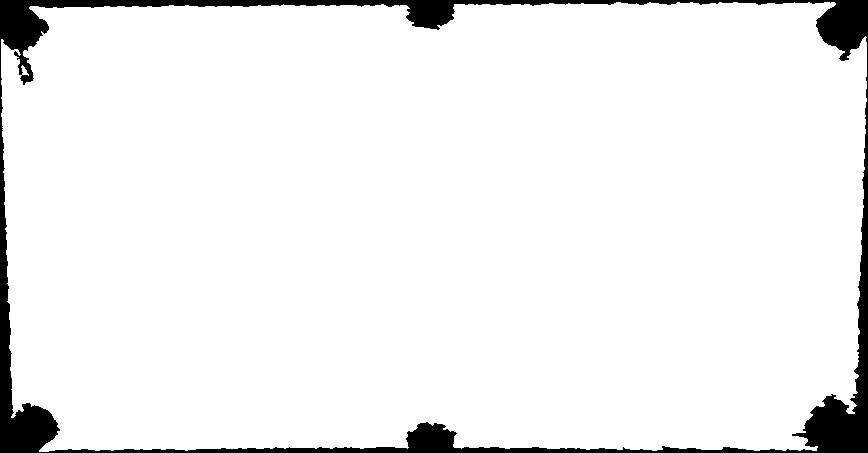
\includegraphics[scale=0.1]{../images/1/8_mask.png}} & A = 368666 & P = 3339 & \multirow{4}{*}{}\\ 
& & & $\lambda$ = 0.9968 & $\kappa$ = 1.0589 & \\
&&&&&\\
&&&&&\\
\hline

\multirow{4}{*}{Lighting III.} & \multirow{4}{*}{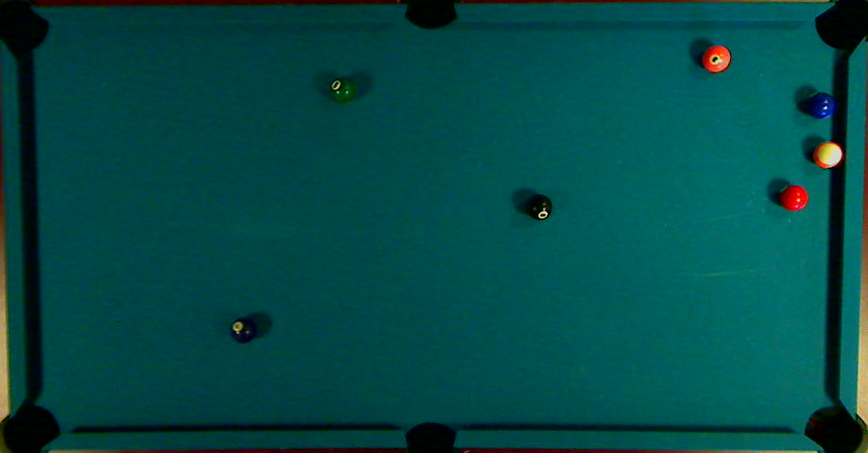
\includegraphics[scale=0.1]{../images/1/14_img.png}} & \multirow{4}{*}{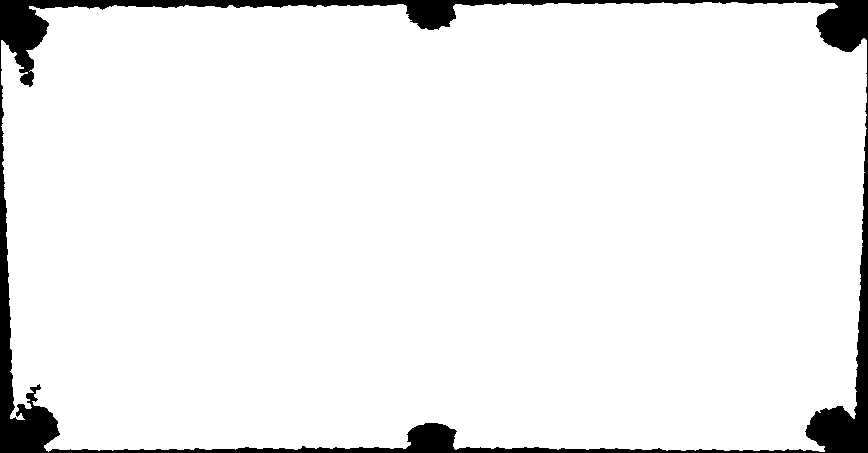
\includegraphics[scale=0.1]{../images/1/14_mask.png}} & A = 368783 & P = 3291 & \multirow{4}{*}{}\\ 
& & & $\lambda$ = 0.9971 & $\kappa$ = 1.0436 & \\
&&&&&\\
&&&&&\\
\hline

\multirow{4}{*}{Lighting IV.} & \multirow{4}{*}{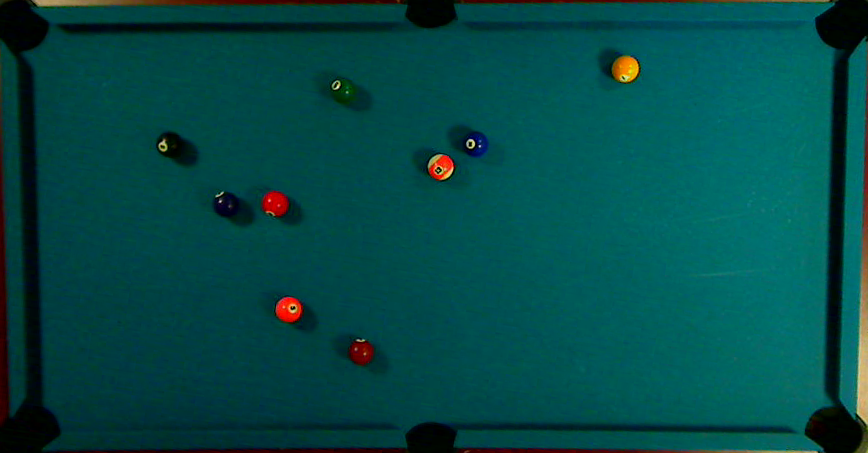
\includegraphics[scale=0.1]{../images/1/9_img.png}} & \multirow{4}{*}{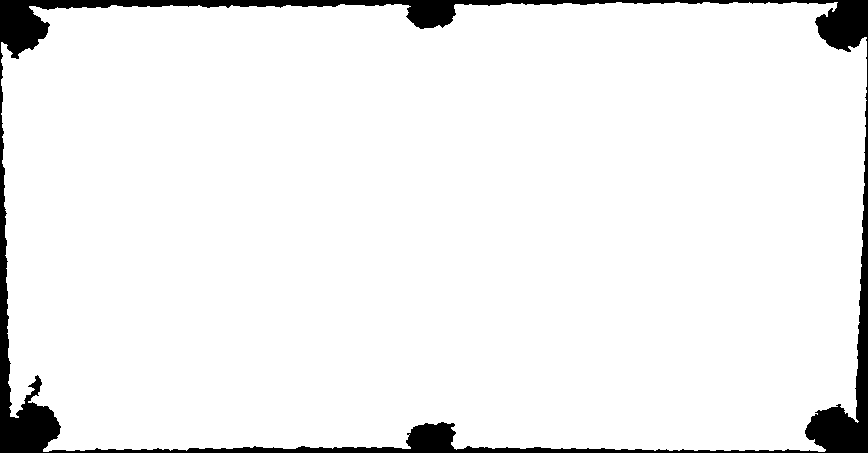
\includegraphics[scale=0.1]{../images/1/9_mask.png}} & A = 369481 & P = 3249 & \multirow{4}{*}{}\\ 
& & & $\lambda$ = 0.9990 & $\kappa$ = 1.0305 & \\
&&&&&\\
&&&&&\\
\hline

\multirow{4}{*}{With ladder.} & \multirow{4}{*}{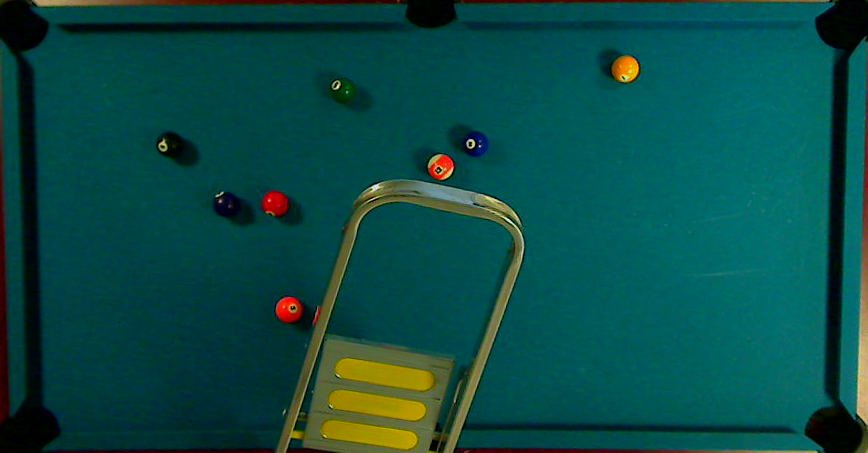
\includegraphics[scale=0.1]{../images/1/10_img.png}} & \multirow{4}{*}{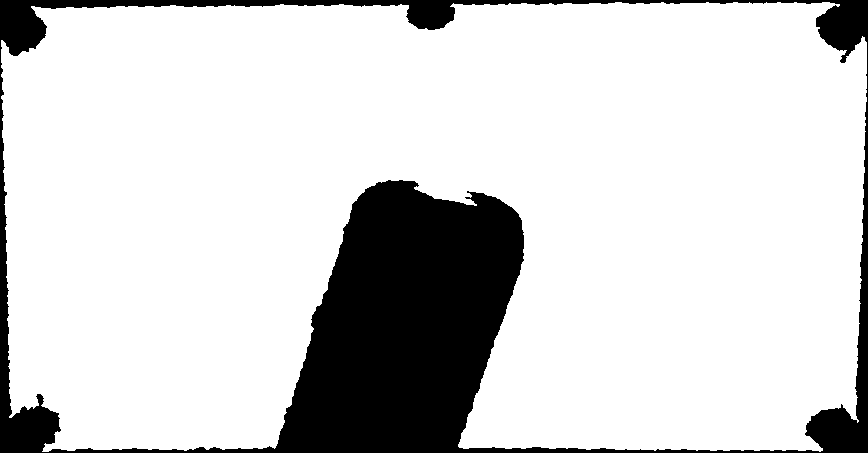
\includegraphics[scale=0.1]{../images/1/10_mask.png}} & A = 324054 & P = 3721 & \multirow{4}{*}{\checkmark}\\ 
& & & $\lambda$ = 0.8762 & $\kappa$ = 1.1801 & \\
&&&&&\\
&&&&&\\
\hline

\multirow{4}{*}{Triangle on table.} & \multirow{4}{*}{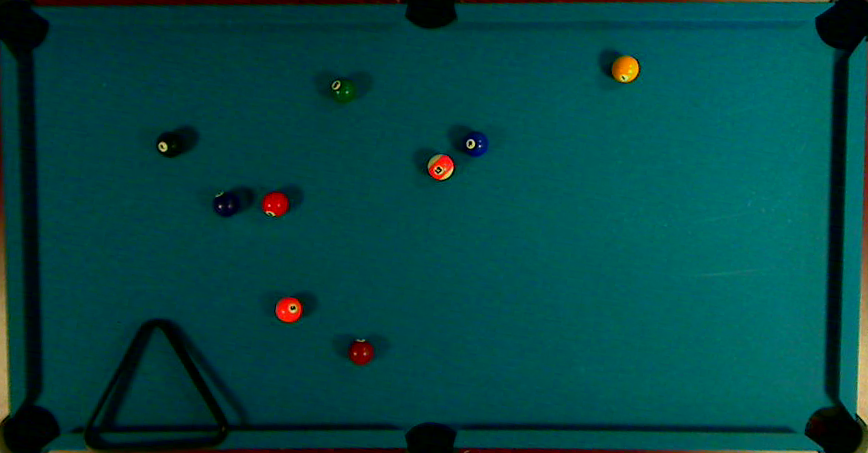
\includegraphics[scale=0.1]{../images/1/13_img.png}} & \multirow{4}{*}{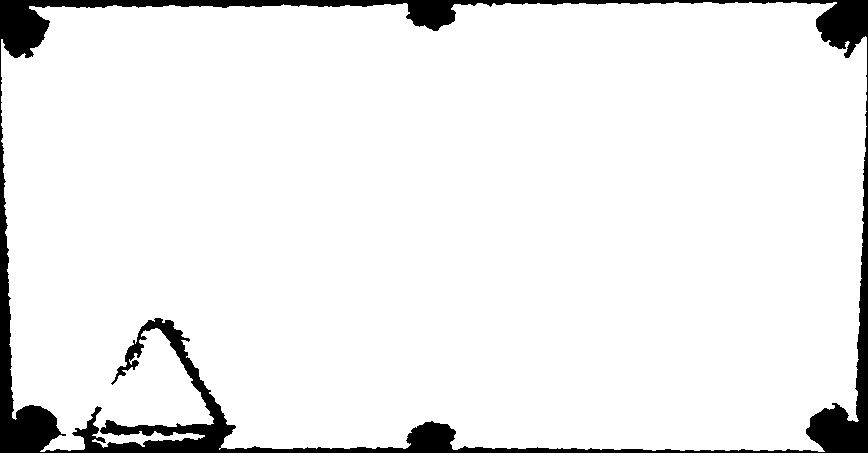
\includegraphics[scale=0.1]{../images/1/13_mask.png}} & A = 364360 & P = 4243 & \multirow{4}{*}{\checkmark}\\ 
& & & $\lambda$ = 0.9851 & $\kappa$ = 1.3456 & \\
&&&&&\\
&&&&&\\
\hline

\multirow{4}{*}{Hand on table.} & \multirow{4}{*}{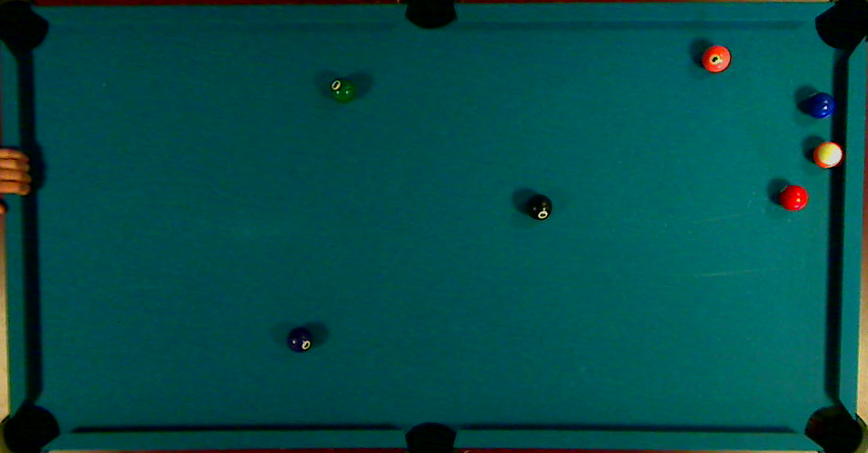
\includegraphics[scale=0.1]{../images/1/15_img.png}} & \multirow{4}{*}{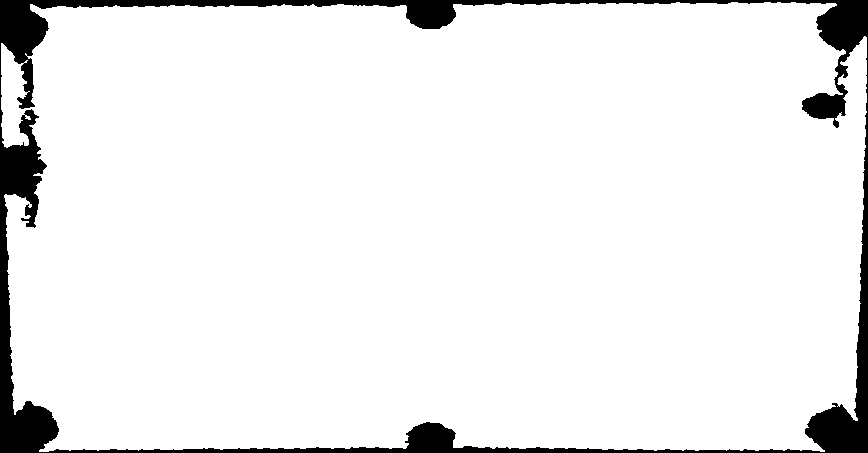
\includegraphics[scale=0.1]{../images/1/15_mask.png}} & A = 364787 & P = 3895 & \multirow{4}{*}{\checkmark}\\ 
& & & $\lambda$ = 0.9863 & $\kappa$ = 1.2351 & \\
&&&&&\\
&&&&&\\
\hline

\end{tabular} 

\textbf{Plot Of Factors:}\\
The plot can be seen in \ref{fig:occlusion_plot}. It does not contain "Lighting I" factors since the perimeter is very high compared to the normal. This is due to the light being altered too much which is not allowed as written in the requirement specification in section \ref{sec:reqspec}.

\begin{figure}[H]
\begin{center}
\leavevmode
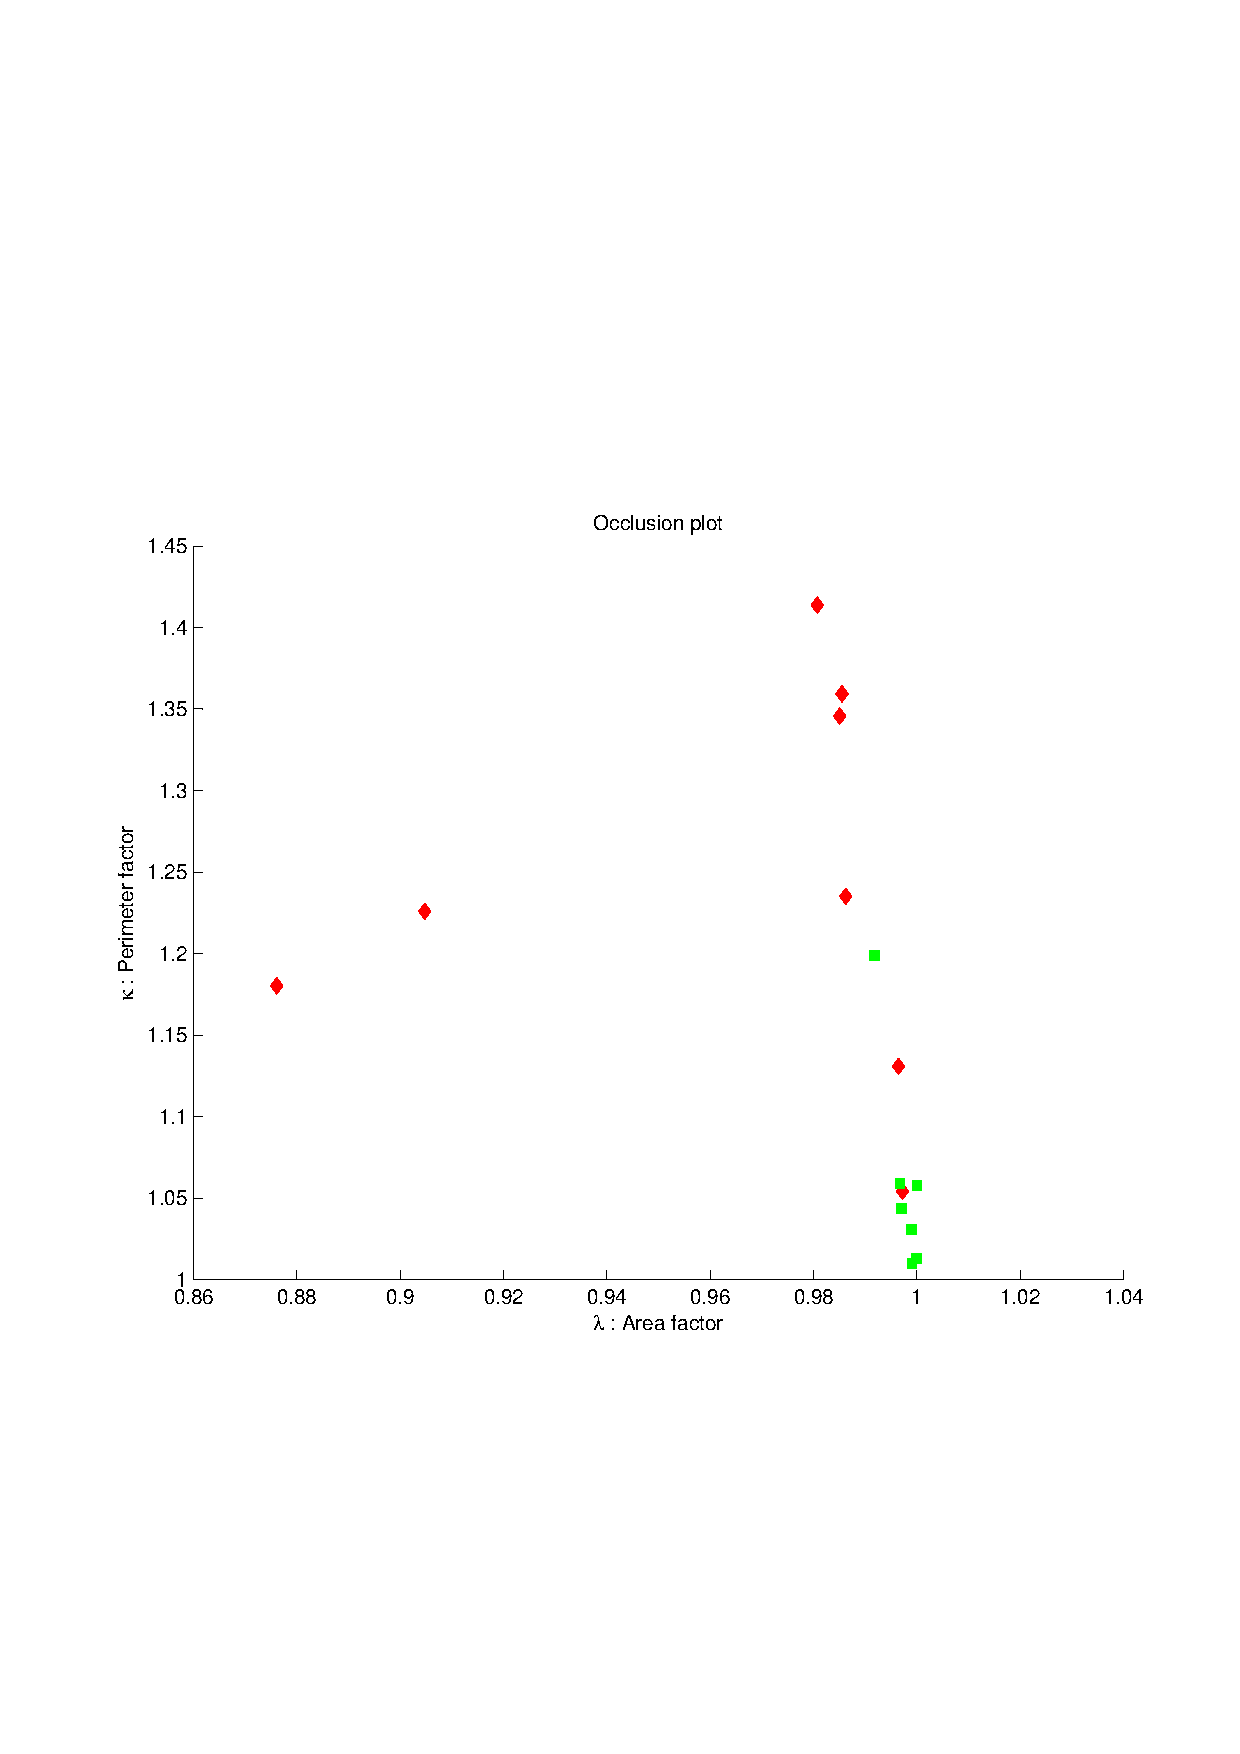
\includegraphics[width=0.7\textwidth]{images/occlusion_plot}
\end{center}
\caption{Occlusion plot. Red triangles are occlusions and green squares are not.}
\label{fig:occlusion_plot}
\end{figure}

The red triangle (occlusion) that lie within the green square (non occlusion) is "Que on table II" which is occlusion by a small part of the que.\\

The green square (non occlusion) that lie between two red diamonds (occlusions) is "Shadow" where a shadow is introduced by a person. This was done while also changing the light. The area factor is very close to normal, but the perimeter is not due to significant light changes underneath the left cushion.\\

The following mean-values have been calculated for the non occlusions:\\

$\mu_{\lambda} = 0.99$\\
$\mu_{\kappa} = 1.06$\\

The occlusion detection is only done to determine if the balls position should be re-evaluated. Therefore it is not crucial that the detection is 100\% correct. A wrong detection will simply cause a re-evaluation of the balls position which would show no movement. Therefore it is optimal to make a "paranoid" classifier that would be more inclined to assume a occlusion than not.\\

Since an introduction of a foreign object will always make the contour area smaller and the perimeter bigger the values for a detection will be set to:

\begin{center}
$\lambda_{detection} if \lambda < 0.99$ \\
or\\
$\kappa_{detection} if \kappa > 1.04$.
\end{center}

Instead of a decision tree, a linear discriminant function could have been made. The outcome is roughly the same and for easier simplification a decision tree was chosen.

\subsection{Ball Movement Detection}
After an human interaction it is required to detect if movement of the balls or change in number of ball is present. If this is the case the 
positions of the balls are saved as a new state. If it is not the case the system will wait for the next human interaction. To detect if movement or number has changed the current number of balls and their positions will be compared to the last saved state. However first it is important to detect if the balls are laying still.

\subsubsection{Distance Measure}
The distances will be calculated using the manhatten distance measure which is defined in equation \ref{eq:manhatten}. The manhatten distance measure has lower complexity than other distances measures which could also have been used and is therefore chosen. 

\begin{equation}
L_{1} = \parallel x_{1}-x_{2}\parallel + \parallel y_{1}-y_{2}\parallel.
\label{eq:manhatten}
\end{equation}

\subsubsection{Detect If Balls Are Laying Still}
Before comparing the positions and number of balls it is important that the balls are laying still, since the focus of the project is based on non-moving ball and a moving balls could give wrong identification due to motion blur, interlacing and so on. This will be done by finding the position of the balls in the current frame and then comparing it to a number of past frames as illustrated in figure \ref{fig:manyframes}.

\begin{figure}[H]
\begin{center}
\leavevmode
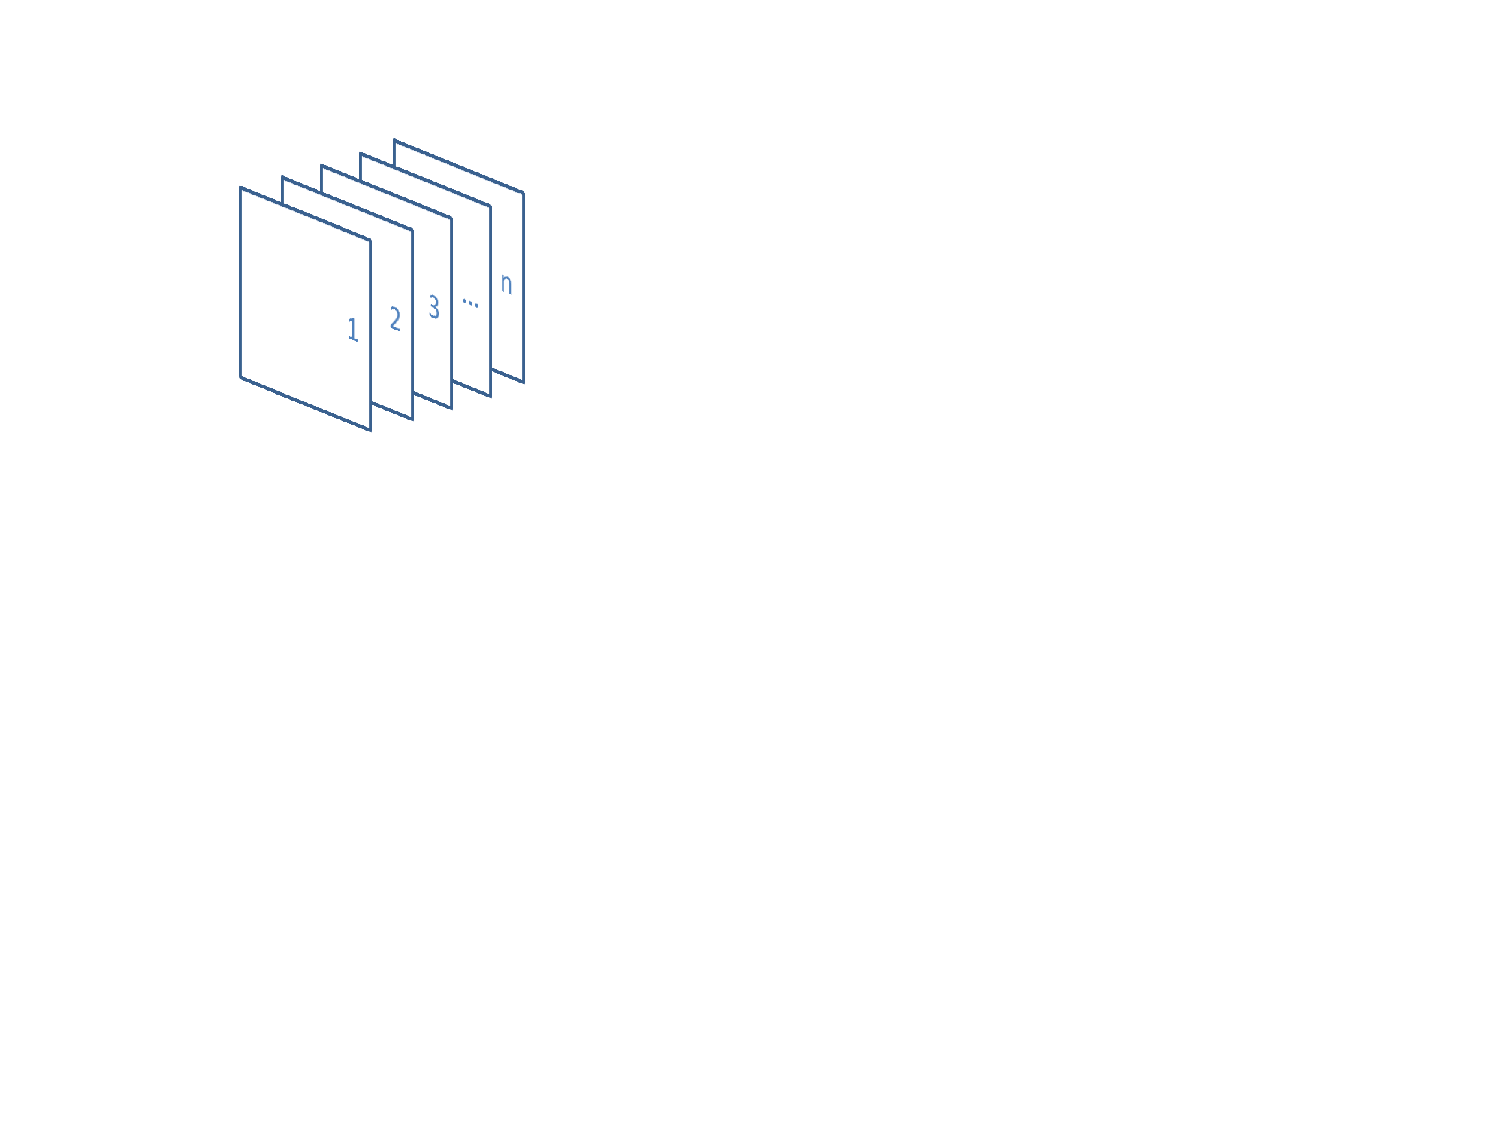
\includegraphics[width=0.5\textwidth]{images/image_seq_numbers}
\end{center}
\caption{Frame one is the current frame, and the rest are past frames.}
\label{fig:manyframes}
\end{figure}

The number of frames in which the balls are laying still should be set on the basis of frames pr. second and the minimal speed of a ball. The number of frames will be decided, dynamically, by equation \ref{eq:dynamiceq}.

\begin{equation}
N = FPS * seconds
\label{eq:dynamiceq}
\end{equation}

If the position of the balls is the same in N frames the balls are laying still. The number of seconds is chosen to be 0.5 s. 

\subsubsection{Movement From Last Saved State.}
To detect if there has been movement of the balls from the last saved state, the current positions will be compared to the positions of the last saved state. This will be done using the chosen distance measurement and a threshold. The threshold will have to be set to a level where noise and shadows does not indicate a new position.\\

The threshold will be set as the radius of a ball, in pixels. If a ball has moved more than this from the last saved state it will be a new state.

\subsubsection{Change In Number Of Balls}
If the number of found balls is different from the number of found balls in the last saved state a new state will be saved with the found positions and colors.\\